\renewcommand{\thefootnote}{\fnsymbol{footnote}}

\chapter[Expected utility theory]%
 {Expected utility theory}
\label{ch:L2}

% 3) Reset things so later footnotes go back to 1, 2, 3, …
%\setcounter{footnote}{0}
\renewcommand{\thefootnote}{\arabic{footnote}}

\section{Assumptions on preferences}\label{sec:L2-intro}

We now impose properties on preferences over lotteries. But first, a brief methodological aside on what we are doing. Before discussing properties of \( \succsim \), we should explicit what the interpretation of \( \succsim \) is. Different methodological stances are possible. Is \( \succsim \) tracking what an individual has in mind? What he would say if asked? How he chose in the past?

Under \textit{revealed preference theory}, we interpret \( \succsim \) as a description of how an individual \textbf{chooses}. Therefore, there is no psychological content to \( \succsim \). Revealed preference theory has been the standard methodological stance in economics for a long time. But why? Wouldn't it be better to develop a theory that exploits psychological insights? Revealed preference theory is exclusively a methodological stance, not a psychological (or, for what matters, a moral) one. The assumption is not that choices are not driven by psychological motives, but that we abstract from these motives and attempt to find patterns in choices directly. There is a strong advantage in doing so: psychological motives are hard to observe, while choices can be observed easily. The implication is that a choice theory based on revealed preferences is more easily testable: if we observe choices that violate the assumptions of the theory, we can reject it. Therefore, revealed preference theory is \textbf{not} a stance on how individuals make choices or what matters for choices, on the contrary, it is silent about these issues.\footnote{If you are interested, you can read \cite{thomaDefenceRevealedPreference2021} for a discussion of the current status of revealed preference theory.} This is often misunderstood: there is a plethora of critics claiming that economics views individuals as cold robots.\footnote{By the way, if you read Asimov's books you now that robots are not cold at all!}

Such critics mostly come from behavioural economics, which is a field that attempts to incorporate psychological insights into economic models.\footnote{In \cite{spieglerCuriousCultureEconomic2024a} you can find a view of the motivations of the founding fathers of behavioural economics.} Is it therefore impossible to do behavioural economics under the revealed preference approach? Not at all. Good behavioural theories do what the name of the field suggests: characterise the behavioural content of the theory, so that, as economist, we know how different individuals behave. Two behavioural theories with different psychological content that are observationally equivalent, i.e., they make the same predictions about choices, are not equally useful for economists.\footnote{There is a huge debate on this topic. Among many, I suggest you to read \cite{gulCaseMindlessEconomics2011} and the response by \cite{camererCaseMindfulEconomics2008}. A more recent piece is \cite{spieglerBehavioralEconomicsAtheoretical2019}.}

\begin{techremark}
	An interesting case study is \cite{masatliogluBehavioralAnalysisStochastic2016}, where the authors show that the famous model by \cite{koszegiReferencedependentRiskAttitudes2007} is behaviourally equivalent to the intersection of rank-dependent utility and quadratic utility, two older models. Another example that is quite relevant today is in \cite{eliazCanAnticipatoryFeelings2006}.
\end{techremark}

In what follows, you can have in mind the interpretation of \( \succsim \) that you prefer, but remember that it is important to be clear about it.

Before discussing the properties of preferences over lotteries, let's consider a reasonable functional form for preferences. A natural candidate is the following: the utility of a lottery \( p \) is given by

\begin{equation}\label{eq:eu}
	\sum_{x\in X} p(x)u(x)
\end{equation}

for some function \( u \colon X \to \mathbb{R} \), assigning to each outcome \( x \) a number representing its utility \( u (x ) \). The idea is simple, the outcome \( x \) realises with probability \( p \), and when \( x \) realises, the individual gets utility \( u(x) \). The functional form in Equation \eqref{eq:eu} is called \textbf{expected utility}. This is because it is the expectation, computed with the probability \( p \), of the utility the individual gets. Before turning to the properties of preferences that will lead us to this functional form, let's make some observations.

Having expected utility preferences over lotteries implies that indifference curves on the simplex are straight lines. That is, say that \( p \sim q \). Then, for any \( \alpha \in (0,1) \) it holds that \( \alpha p + (1-\alpha) q \sim p \), as illustrate in Figure \ref{fig:simplex-ind}.

\begin{figure}[H]
	\centering
	% \usetikzlibrary{calc} % <-- enable if you keep the ($(P)!t!(Q)$) syntax
	\begin{tikzpicture}[scale=1]
		% small filled dot style
		\tikzset{dot/.style={circle,fill,inner sep=1.4pt}}

		%--- simplex vertices --------------------------------------------------------
		\coordinate (A) at (0,0);
		\coordinate (B) at (6,0);
		\coordinate (C) at (3,5.196); % = (sqrt(3)/2)*6

		\draw[thick] (A)--(B)--(C)--cycle;

		% vertex labels = degenerate lotteries
		\node[dot] at (A) {};
		\node[below,align=center] at (A) {$x$ \\ {\scriptsize $(1,0,0)$}};
		\node[dot] at (B) {};
		\node[below,align=center] at (B) {$y$ \\ {\scriptsize $(0,1,0)$}};
		\node[dot] at (C) {};
		\node[above,align=center] at (C) {{\scriptsize $(0,0,1)$}\\[-2pt] $z$};

		%--- two interior lotteries p and q -----------------------------------------
		\coordinate (P) at (1.7,1.35);
		\coordinate (Q) at (4.2,1.15);

		\node[dot] at (P) {};
		\node[above left=2pt] at (P) {$p$};

		\node[dot] at (Q) {};
		\node[above right=2pt] at (Q) {$q$};

		% segment of mixtures r_λ = λ p + (1-λ) q  (indifference set if p ~ q)
		\draw[very thick] (P)--(Q);

		% an example interior mixture point on the segment
		\coordinate (R) at ($(P)!0.42!(Q)$); % requires calc library
		\node[below=3pt] at (R) {$\alpha p+(1-\alpha)q$};

	\end{tikzpicture}
	\caption{If \( p \sim q \), then any mixture of \( p \) and \( q \) is also indifferent to \( p \) and \( q \).}
	\label{fig:simplex-ind}
\end{figure}

Let's show this formally. Assume that \( p \sim q \). Then, by definition of expected utility, we have

\[
	\sum_{x\in X} p(x)u(x) = \sum_{x\in X} q(x)u(x).
\]

By applying expected utility again, for any \( \alpha \in (0,1) \), the utility of the lottery \( \alpha p + (1-\alpha) q \) is given by

\begin{align*}
	\sum_{x\in X} \big(\alpha p(x) + (1-\alpha) q(x)\big) u(x)
	 & = \sum_{x\in X} \alpha p(x) u(x) + \sum_{x\in X} (1-\alpha) q(x) u(x) \\
	 & = \alpha \sum_{x\in X} p(x) u(x) + (1-\alpha) \sum_{x\in X} q(x) u(x) \\
	 & = \alpha \sum_{x\in X} q(x) u(x) + (1-\alpha) \sum_{x\in X} q(x) u(x) \\
	 & = \sum_{x\in X} q(x) u(x).
\end{align*}

Indifference curves are also parallel, you are asked to show this in Exercise \ref{ex:parallel-lines}.

Let's now turn to the properties of \( \succsim \) we will consider. First, we assume that preferences are a \textbf{weak order}.

\begin{axiom}\label{ax:wo}
	\labelname{axn:wo}{Weak order} (\textbf{Weak order}) Preferences \(\succsim\) are complete and transitive.
\end{axiom}

Recall that preferences are \textbf{complete} if for any two lotteries \(p,q\), either \(p\succsim q\) or \(q\succsim p\), or both. They are transitive if for any three lotteries \(p,q,r\), if \(p\succsim q\) and \(q\succsim r\), then \(p\succsim r\).

\begin{axiom}\label{ax:continuity}
	\labelname{axn:continuity}{Continuity} (\textbf{Continuity}) For any three lotteries \(p,q,r\), if \(p\succ q\succ r\) then there exist \(\alpha,\beta\in(0,1)\) such that \(\alpha p+(1-\alpha)r\succ q\succ \beta p+(1-\beta)r\).
\end{axiom}

\begin{axiom}
	\labelname{axn:independence}{Independence} (\textbf{Independence}) For any three lotteries \(p,q,r\) and for any \(\alpha\in(0,1)\), we have \( p \succsim q \) if and only if \(\alpha p+(1-\alpha)r\succsim \alpha q+(1-\alpha)r\).
\end{axiom}

\begin{lemma}
	Let \( \succsim \) satisfy \usename{axn:wo}, \usename{axn:continuity}, and \usename{axn:independence}, then there exist two lotteries \( \overline p \) and
	\( \underline p \) such that \( \overline p \succsim p \succsim \underline p \) \text{for all} \( p \).
\end{lemma}

\begin{proof}
	The proof is in two steps.

	\paragraph{Step 1.} By \usename{axn:wo}, the restriction of \( \succsim \) to the set of lotteries giving positive probability to only one outcome \( \{\delta_x: x\in X\} \) is a complete and transitive order on a \emph{finite} set. Hence there exist $x^\ast,x_\ast$ such that

	\[
		\delta_{x^\ast} \succsim \delta_x \succsim \delta_{x_\ast} \qquad\text{for all } x .
	\]

	Fix \( \overline p:=\delta_{x^\ast}\) and \(\underline p:=\delta_{x_\ast}\).

	\paragraph{Step 2.} For \( p\in \Delta(X) \) write \( supp(p)=\{x\in Z: p(x)>0\} \) and let \(|supp(p)|\) be its size. We prove by induction on \(k:=|supp(p)|\) that

	\[
		\overline p \succsim p \succsim \underline p .
	\]

	\emph{Base case $k=1$.}
	If $supp(p)=\{x\}$, then $p=\delta_x$ and the claim follows from Step~1.

	\emph{Inductive step.}
	Assume the statement holds for all lotteries with support size $\le k-1$.
	Let $p$ have support size $k\ge2$. Pick any $x \in supp(p)$ and write
	\[
		p \;=\; \lambda\,\delta_x + (1-\lambda)\,q,
		\qquad \lambda:=p(x)\in(0,1),
	\]
	where $q$ is the renormalized remainder (so $|supp(q)|\le k-1$).

	By the inductive hypothesis, $\overline p \succsim q$; by Step~1, $\overline p \succsim \delta_x$.
	Using Independence twice and transitivity,
	\[
		\overline p
		~\succsim~ \lambda\,\overline p + (1-\lambda)\,q
		~\succsim~ \lambda\,\delta_x + (1-\lambda)\,q
		~=~ p .
	\]
	(The first relation comes from $\overline p \succsim q$ with $t=1-\lambda$ and $Z=\overline p$;
	the second from $\overline p \succsim \delta_x$ with $t=\lambda$ and $Z=q$.)

	A symmetric argument gives $p \succsim \underline p$:
	by the inductive hypothesis $q \succsim \underline p$ and by Step~1 $\delta_x \succsim \underline p$;
	then, by Independence and transitivity,
	\[
		p=\lambda\,\delta_x+(1-\lambda)\,q
		~\succsim~ \lambda\,\underline p+(1-\lambda)\,q
		~\succsim~ \underline p .
	\]

	Thus $\overline p \succsim p \succsim \underline p$ for all lotteries with support size $k$,
	closing the induction.

	\medskip
	Therefore, the fixed Diracs $\overline p=\delta_{x^\ast}$ and
	$\underline p=\delta_{x_\ast}$ bound every lottery $p\in\Delta(Z)$, as claimed.
\end{proof}


\section{Expected utility representation}

We are ready to state and prove the theorem relating the properties of preferences over lotteries to the expected utility functional form.

\begin{theorem}\label{thm:eu}
	Preferences over lotteries \(\succsim\) satisfy \usename{axn:wo}, \usename{axn:continuity}, \usename{axn:independence} if and only if then there exists a utility function \(u \colon X\to\mathbb{R}\) such that:

	\begin{equation}
		p \succsim q \text{ if and only if } \sum_{x\in X} p(x)u(x) \geq \sum_{x\in X} q(x)u(x).
	\end{equation}

	We say that \(u\) \textbf{represents} \(\succsim\).
\end{theorem}

The proof here essentially follows \citet[pp.~176–178]{mas-colellMicroeconomicTheory1995}, but it is complemented by intuition and figures.

\begin{proof}
	We proceed by steps.

	\paragraph{Step 1.} If \( p \succsim q \) then \( p \succsim \alpha p + (1-\alpha) q \succsim q \) for any \( \alpha \in (0,1) \).

	The intuition behind this step is simple: if \( p \) is better than \( q \), than any mixture between the two is worse than \( p \) and better than \( q \). Figure \ref{fig:step1} illustrates the idea.

	\begin{figure}[H]
		\centering
		\tikzset{every picture/.style={line width=0.75pt}} %set default line width to 0.75pt        

		\begin{tikzpicture}[x=0.65pt,y=0.65pt,yscale=-1,xscale=1]
			%uncomment if require: \path (0,412); %set diagram left start at 0, and has height of 412

			%Shape: Triangle [id:dp7624353544488017] 
			\draw   (292.33,43.07) -- (474.67,369.07) -- (110,369.07) -- cycle ;
			%Straight Lines [id:da31966546289590647] 
			\draw  [dash pattern={on 4.5pt off 4.5pt}]  (262,220.92) -- (398.67,316.25) ;
			%Shape: Circle [id:dp6804955961429688] 
			\draw  [fill={rgb, 255:red, 0; green, 0; blue, 0 }  ,fill opacity=1 ] (396.25,316.25) .. controls (396.25,314.92) and (397.33,313.83) .. (398.67,313.83) .. controls (400,313.83) and (401.08,314.92) .. (401.08,316.25) .. controls (401.08,317.58) and (400,318.67) .. (398.67,318.67) .. controls (397.33,318.67) and (396.25,317.58) .. (396.25,316.25) -- cycle ;
			%Shape: Circle [id:dp44734973339031014] 
			\draw  [fill={rgb, 255:red, 0; green, 0; blue, 0 }  ,fill opacity=1 ] (259.58,220.92) .. controls (259.58,219.58) and (260.67,218.5) .. (262,218.5) .. controls (263.33,218.5) and (264.42,219.58) .. (264.42,220.92) .. controls (264.42,222.25) and (263.33,223.33) .. (262,223.33) .. controls (260.67,223.33) and (259.58,222.25) .. (259.58,220.92) -- cycle ;
			%Curve Lines [id:da39390655998084656] 
			\draw    (330.33,268.58) .. controls (378.93,256.92) and (391.95,237.98) .. (405.07,206.2) ;
			\draw [shift={(405.67,204.74)}, rotate = 112.2] [color={rgb, 255:red, 0; green, 0; blue, 0 }  ][line width=0.75]    (10.93,-3.29) .. controls (6.95,-1.4) and (3.31,-0.3) .. (0,0) .. controls (3.31,0.3) and (6.95,1.4) .. (10.93,3.29)   ;
			%Shape: Circle [id:dp4485716510591613] 
			\draw  [fill={rgb, 255:red, 0; green, 0; blue, 0 }  ,fill opacity=1 ] (327.92,268.58) .. controls (327.92,267.25) and (329,266.17) .. (330.33,266.17) .. controls (331.67,266.17) and (332.75,267.25) .. (332.75,268.58) .. controls (332.75,269.92) and (331.67,271) .. (330.33,271) .. controls (329,271) and (327.92,269.92) .. (327.92,268.58) -- cycle ;

			% Text Node
			\draw (392.67,176.4) node [anchor=north west][inner sep=0.75pt]    {$\alpha p +( 1-\alpha ) q\ $};
			% Text Node
			\draw (254,192.4) node [anchor=north west][inner sep=0.75pt]    {$p$};
			% Text Node
			\draw (406,306.4) node [anchor=north west][inner sep=0.75pt]    {$q$};


		\end{tikzpicture}
		\caption{Step 1.}
		\label{fig:step1}
	\end{figure}

	This follows from \usename{axn:independence}.

	\begin{equation}\label{eq:comp1}
		p \succsim q \implies (1-\alpha) p + \alpha p \succsim (1-\alpha) q + \alpha q \implies p \succsim \alpha p + (1-\alpha) q \succsim q.
	\end{equation}

	\begin{equation}\label{eq:comp2}
		p \succsim q \implies \alpha p + (1-\alpha) q \succsim \alpha q + (1-\alpha) q \implies \alpha p + (1-\alpha) q \succsim q.
	\end{equation}

	The conclusion follows from Equations \eqref{eq:comp1} and \eqref{eq:comp2}.

	\paragraph{Step 2.} \(\beta>\alpha \) if and only if \( \beta \overline{p} +(1-\beta) \underline{p} \succ \alpha \overline{p}+(1-\alpha) \underline{p} \).

	The idea for this step is the following. From \textbf{Step 1}, we know that a mixture between \( p \) and \( q \), where \( p \succsim q \) is better than \( q \) and worse than \( p \). Now, we know that \( \overline{p} \succ \alpha \overline{p} +(1-\alpha) \underline{p}\), since \( \overline{p} \) is the best lottery available. We want to show that \( \beta \overline{p} + (1-\beta) \underline{p} \) is a mixture between \( \overline{p} \) and \( \alpha \overline{p} + (1-\alpha) \underline{p} \), and therefore, by \textbf{Step 1}, better than \( \alpha \overline{p} + (1-\alpha) \underline{p} \). The idea is illustrated in Figure \ref{fig:step2}.

	\begin{figure}[H]
		\centering
		\tikzset{every picture/.style={line width=0.75pt}} %set default line width to 0.75pt        
		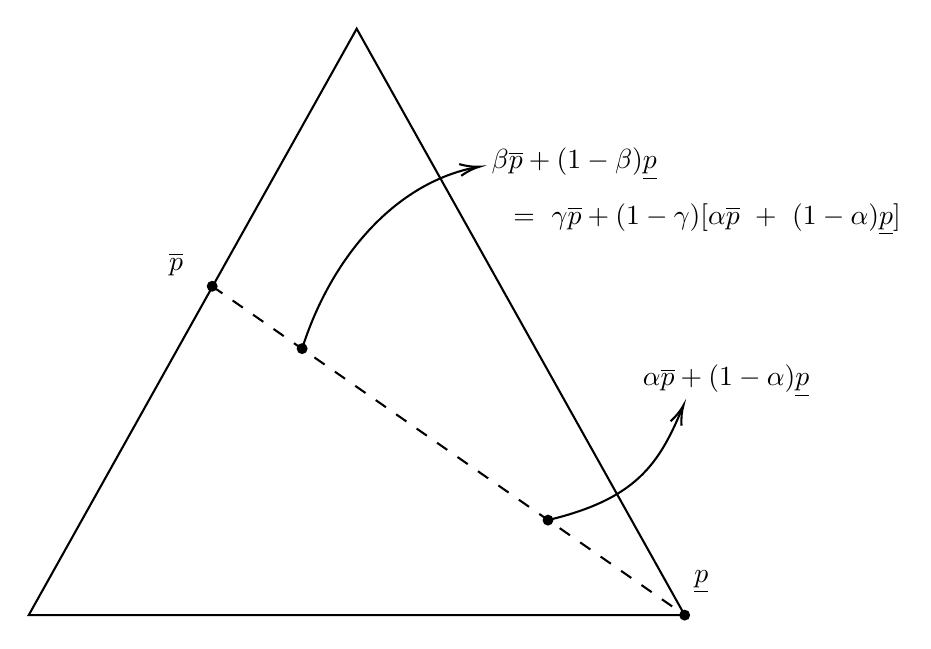
\begin{tikzpicture}[x=0.65pt,y=0.65pt,yscale=-1,xscale=1]
			%uncomment if require: \path (0,376); %set diagram left start at 0, and has height of 376
			%Shape: Triangle [id:dp5718796353912894] 
			\draw   (329.33,23.07) -- (511.67,349.07) -- (147,349.07) -- cycle ;
			%Shape: Circle [id:dp9404346697828574] 
			\draw  [fill={rgb, 255:red, 0; green, 0; blue, 0 }  ,fill opacity=1 ] (509.25,349.07) .. controls (509.25,347.74) and (510.33,346.66) .. (511.67,346.66) .. controls (513,346.66) and (514.08,347.74) .. (514.08,349.07) .. controls (514.08,350.41) and (513,351.49) .. (511.67,351.49) .. controls (510.33,351.49) and (509.25,350.41) .. (509.25,349.07) -- cycle ;
			%Shape: Circle [id:dp21608178484403062] 
			\draw  [fill={rgb, 255:red, 0; green, 0; blue, 0 }  ,fill opacity=1 ] (246.58,166.25) .. controls (246.58,164.92) and (247.67,163.83) .. (249,163.83) .. controls (250.33,163.83) and (251.42,164.92) .. (251.42,166.25) .. controls (251.42,167.58) and (250.33,168.67) .. (249,168.67) .. controls (247.67,168.67) and (246.58,167.58) .. (246.58,166.25) -- cycle ;
			%Straight Lines [id:da0014271293885499414] 
			\draw  [dash pattern={on 4.5pt off 4.5pt}]  (249,166.25) -- (511.67,349.07) ;
			%Shape: Circle [id:dp09512564117547329] 
			\draw  [fill={rgb, 255:red, 0; green, 0; blue, 0 }  ,fill opacity=1 ] (433.25,296.25) .. controls (433.25,294.92) and (434.33,293.83) .. (435.67,293.83) .. controls (437,293.83) and (438.08,294.92) .. (438.08,296.25) .. controls (438.08,297.58) and (437,298.67) .. (435.67,298.67) .. controls (434.33,298.67) and (433.25,297.58) .. (433.25,296.25) -- cycle ;
			%Shape: Circle [id:dp3186545134308967] 
			\draw  [fill={rgb, 255:red, 0; green, 0; blue, 0 }  ,fill opacity=1 ] (296.58,200.92) .. controls (296.58,199.58) and (297.67,198.5) .. (299,198.5) .. controls (300.33,198.5) and (301.42,199.58) .. (301.42,200.92) .. controls (301.42,202.25) and (300.33,203.33) .. (299,203.33) .. controls (297.67,203.33) and (296.58,202.25) .. (296.58,200.92) -- cycle ;
			%Curve Lines [id:da7950025520809244] 
			\draw    (435.67,296.25) .. controls (484.26,284.58) and (497.28,265.65) .. (510.4,233.87) ;
			\draw [shift={(511,232.41)}, rotate = 112.2] [color={rgb, 255:red, 0; green, 0; blue, 0 }  ][line width=0.75]    (10.93,-3.29) .. controls (6.95,-1.4) and (3.31,-0.3) .. (0,0) .. controls (3.31,0.3) and (6.95,1.4) .. (10.93,3.29)   ;
			%Curve Lines [id:da31359625192132545] 
			\draw    (299,200.92) .. controls (314.84,150.91) and (350.28,108.59) .. (396.27,99.99) ;
			\draw [shift={(397.67,99.74)}, rotate = 170.27] [color={rgb, 255:red, 0; green, 0; blue, 0 }  ][line width=0.75]    (10.93,-3.29) .. controls (6.95,-1.4) and (3.31,-0.3) .. (0,0) .. controls (3.31,0.3) and (6.95,1.4) .. (10.93,3.29)   ;

			% Text Node
			\draw (223.33,146.07) node [anchor=north west][inner sep=0.75pt]    {$\overline{p}$};
			% Text Node
			\draw (515.33,322.4) node [anchor=north west][inner sep=0.75pt]    {$\underline{p}$};
			% Text Node
			\draw (486.67,208.4) node [anchor=north west][inner sep=0.75pt]    {$\alpha \overline{p} +( 1-\alpha )\underline{p} \ $};
			% Text Node
			\draw (402.67,87.73) node [anchor=north west][inner sep=0.75pt]    {$\beta \overline{p} +( 1-\beta )\underline{p} \ $};
			% Text Node
			\draw (414.67,118.73) node [anchor=north west][inner sep=0.75pt]    {$=\ \gamma \overline{p} +( 1-\gamma )[ \alpha \overline{p} \ +\ ( 1-\alpha )\underline{p}]$};


		\end{tikzpicture}
		\caption{Step 2.}
		\label{fig:step2}
	\end{figure}

	We want to write \( \beta \overline{p} + (1-\beta) \underline{p} \) as a mixture between \( \overline{p} \) and \( \alpha \overline{p} + (1-\alpha) \underline{p} \). That is, we want to find \( \gamma \in (0,1) \) such that

	\[
		\beta \overline{p} + (1-\beta) \underline{p} = \gamma \overline{p} + (1-\gamma)[\alpha \overline{p} + (1-\alpha) \underline{p}].
	\]

	With some algebra we get that \( \gamma = \frac{\beta - \alpha}{1 - \alpha} \). By step 1 we know that \( \overline{p} \succ \alpha \overline{p} + (1-\alpha) \underline{p} \), therefore, \( \gamma \overline{p} + (1-\gamma)[\alpha \overline{p} + (1-\alpha) \underline{p}] \succ \alpha \overline{p} + (1-\alpha) \underline{p} \). Since \( \beta \overline{p} + (1-\beta) \underline{p} = \gamma \overline{p} + (1-\gamma)[\alpha \overline{p} + (1-\alpha) \underline{p}] \), the conclusion follows.

	Until now we proved that if \( \beta > \alpha \) then \( \beta \overline{p} + (1-\beta) \underline{p} \succ \alpha \overline{p} + (1-\alpha) \underline{p} \). But the statement says \textquote{if and only if}, so we have to prove that if \( \alpha \geq \beta \) then it is not the case that \( \beta \overline{p} + (1-\beta) \underline{p} \succ \alpha \overline{p} + (1-\alpha) \underline{p} \). When \( \beta = \alpha \) the two are the same lotteries and therefore are indifferent. The relevant case is when \( \alpha > \beta \). By the argument above, we know that \( \alpha \overline{p} + (1-\alpha) \underline{p} \succ \beta \overline{p} + (1-\beta) \underline{p} \), and that's all.

	\paragraph{Step 3.}\footnote{In this step we make use of proof by contradiction. Before diving in, you should make sure your are familiar with the logic of such proofs.} For any \( p \), there exists a unique \( \alpha_p \in [0,1] \) such that \( p \sim \alpha_p \overline{p} + (1-\alpha_p) \underline{p} \).

	We can derive this step as an implication of previous steps and \usename{axn:continuity}. Unfortunately, this step requires a bit of algebra. But you can get some intuition from Figure \ref{fig:step3}.

	\begin{figure}[H]
		\centering
		\tikzset{every picture/.style={line width=0.75pt}} %set default line width to 0.75pt        
		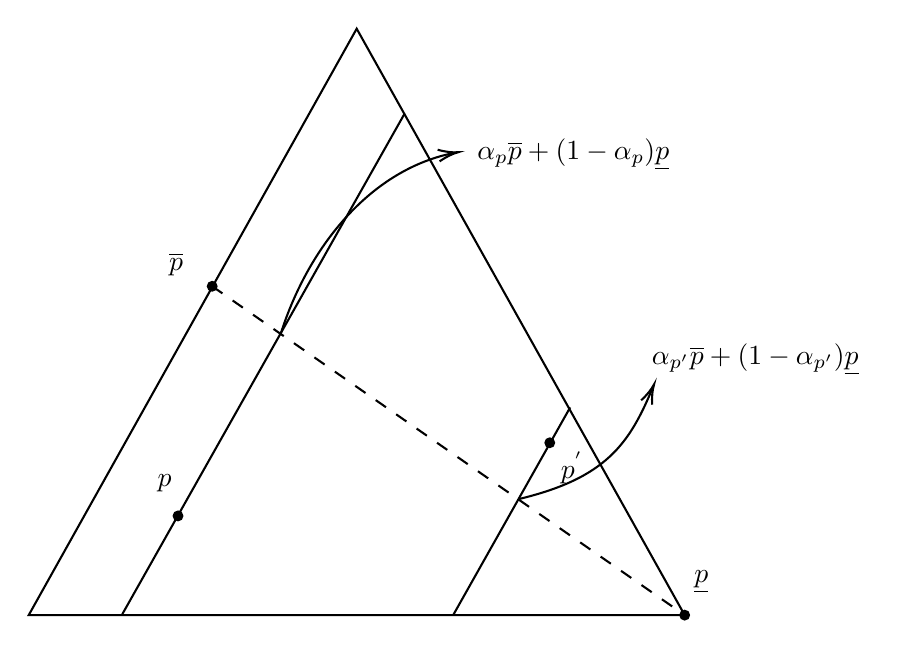
\begin{tikzpicture}[x=0.65pt,y=0.65pt,yscale=-1,xscale=1]
			%uncomment if require: \path (0,426); %set diagram left start at 0, and has height of 426

			%Shape: Triangle [id:dp8490740112879205] 
			\draw   (284.33,42.07) -- (466.67,368.07) -- (102,368.07) -- cycle ;
			%Shape: Circle [id:dp35031725224734067] 
			\draw  [fill={rgb, 255:red, 0; green, 0; blue, 0 }  ,fill opacity=1 ] (464.25,368.07) .. controls (464.25,366.74) and (465.33,365.66) .. (466.67,365.66) .. controls (468,365.66) and (469.08,366.74) .. (469.08,368.07) .. controls (469.08,369.41) and (468,370.49) .. (466.67,370.49) .. controls (465.33,370.49) and (464.25,369.41) .. (464.25,368.07) -- cycle ;
			%Shape: Circle [id:dp5994426130925808] 
			\draw  [fill={rgb, 255:red, 0; green, 0; blue, 0 }  ,fill opacity=1 ] (201.58,185.25) .. controls (201.58,183.92) and (202.67,182.83) .. (204,182.83) .. controls (205.33,182.83) and (206.42,183.92) .. (206.42,185.25) .. controls (206.42,186.58) and (205.33,187.67) .. (204,187.67) .. controls (202.67,187.67) and (201.58,186.58) .. (201.58,185.25) -- cycle ;
			%Straight Lines [id:da10409961384235067] 
			\draw  [dash pattern={on 4.5pt off 4.5pt}]  (204,185.25) -- (466.67,368.07) ;
			%Shape: Circle [id:dp20798560554542445] 
			\draw  [fill={rgb, 255:red, 0; green, 0; blue, 0 }  ,fill opacity=1 ] (389.25,272.25) .. controls (389.25,270.92) and (390.33,269.83) .. (391.67,269.83) .. controls (393,269.83) and (394.08,270.92) .. (394.08,272.25) .. controls (394.08,273.58) and (393,274.67) .. (391.67,274.67) .. controls (390.33,274.67) and (389.25,273.58) .. (389.25,272.25) -- cycle ;
			%Shape: Circle [id:dp4192734085033405] 
			\draw  [fill={rgb, 255:red, 0; green, 0; blue, 0 }  ,fill opacity=1 ] (182.58,312.92) .. controls (182.58,311.58) and (183.67,310.5) .. (185,310.5) .. controls (186.33,310.5) and (187.42,311.58) .. (187.42,312.92) .. controls (187.42,314.25) and (186.33,315.33) .. (185,315.33) .. controls (183.67,315.33) and (182.58,314.25) .. (182.58,312.92) -- cycle ;
			%Straight Lines [id:da3902197637661603] 
			\draw    (154,367.6) -- (311,89.2) ;
			%Straight Lines [id:da7454732907488841] 
			\draw    (338,368) -- (403,252.6) ;
			%Curve Lines [id:da5696173015502568] 
			\draw    (242,211.92) .. controls (257.84,161.91) and (293.28,119.59) .. (339.27,110.99) ;
			\draw [shift={(340.67,110.74)}, rotate = 170.27] [color={rgb, 255:red, 0; green, 0; blue, 0 }  ][line width=0.75]    (10.93,-3.29) .. controls (6.95,-1.4) and (3.31,-0.3) .. (0,0) .. controls (3.31,0.3) and (6.95,1.4) .. (10.93,3.29)   ;
			%Curve Lines [id:da32978400124499274] 
			\draw    (374.33,303.58) .. controls (422.93,291.92) and (435.95,272.98) .. (449.07,241.2) ;
			\draw [shift={(449.67,239.74)}, rotate = 112.2] [color={rgb, 255:red, 0; green, 0; blue, 0 }  ][line width=0.75]    (10.93,-3.29) .. controls (6.95,-1.4) and (3.31,-0.3) .. (0,0) .. controls (3.31,0.3) and (6.95,1.4) .. (10.93,3.29)   ;

			% Text Node
			\draw (178.33,165.07) node [anchor=north west][inner sep=0.75pt]    {$\overline{p}$};
			% Text Node
			\draw (470.33,341.4) node [anchor=north west][inner sep=0.75pt]    {$\underline{p}$};
			% Text Node
			\draw (349.67,101.4) node [anchor=north west][inner sep=0.75pt]    {$\alpha _{p}\overline{p} +( 1-\alpha _{p})\underline{p} \ $};
			% Text Node
			\draw (172,288.4) node [anchor=north west][inner sep=0.75pt]    {$p$};
			% Text Node
			\draw (396.08,275.65) node [anchor=north west][inner sep=0.75pt]    {$p^{'}$};
			% Text Node
			\draw (446.67,215.4) node [anchor=north west][inner sep=0.75pt]    {$\alpha _{p'}\overline{p} +( 1-\alpha _{p'})\underline{p} \ $};


		\end{tikzpicture}
		\caption{Step 3.}
		\label{fig:step3}
	\end{figure}

	First, notice that if \( \alpha_p \) exists, it must be unique. Suppose there are two such numbers \( \alpha_p \) and \( \alpha_p' \) with \( \alpha_p > \alpha_p' \), then by Step 2, \( \alpha_p \overline{p} + (1-\alpha_p) \underline{p} \succ \alpha_p^{\prime} \overline{p} + (1-\alpha_p^{\prime}) \underline{p} \), contradicting indifference to \( p \).

	Now we have to show that such \( \alpha_p \) exists. If \( \overline{p} \sim p \) then \( \alpha_p = 1 \) works, and if \( \underline{p} \sim p \) then \( \alpha_p = 0 \) works. So we have to look at the interesting case \( \overline{p} \succ p \succ \underline{p} \).

	Define

	\begin{equation}\label{eq:astar}
		\alpha_p \;=\; \sup \bigl\{\alpha\in[0,1]\;:\; p \succsim \alpha \overline{p} + (1-\alpha) \underline{p}\bigr\}.
	\end{equation}

	Since \( \alpha = 0 \) is in this set, we are sure that the supremum is not over an empty set.

	We now have to do a few algebraic arguments.

	\begin{equation}\label{eq:claim0}
		\text{If} \: \:  1\ge \alpha >\alpha_p \: \: \text{then} \: \: \alpha \overline{p}+(1-\alpha)\underline{p} \succ p .
	\end{equation}

	Indeed, if \(p\succsim \alpha\overline{p}+(1-\alpha)\underline{p}\) held for such \(\alpha \), then \(\alpha_p \) would not satisfy Equation \eqref{eq:astar}. Moreover:

	\begin{equation}\label{eq:claim1}
		\text{If} \: \: 0\le \alpha<\alpha_p \: \: \text{then} \: \: p \succ \alpha\overline{p}+(1-\alpha)\underline{p}.
	\end{equation}

	The reason is as follows. By the definition of \( \alpha_p \), there exists \(\alpha'\) such that \(\alpha<\alpha'\le \alpha_p\) and \(p\succsim \alpha'\overline{p}+(1-\alpha')\underline{p}\). Since \( \alpha < \alpha' \), \textbf{Step 2} implies that \( p \succ \alpha'\overline{p}+(1-\alpha')\underline{p} \succ \alpha \overline{p} + (1-\alpha)\underline{p} \).

	Now,there are three possibilities to consider:  \( \alpha_p \overline{p} + (1-\alpha_p) \underline{p} \succ p\), \( p\succ \alpha_p \overline{p} + (1-\alpha_p) \underline{p} \), or they are indifferent. If \( \alpha_p \overline{p} + (1-\alpha_p) \underline{p} \succ p\), by \usename{axn:continuity} there exists \(\beta\in(0,1)\) such that \( \beta\bigl(\alpha_p \overline{p} + (1-\alpha_p)\underline{p}\bigr) + (1-\beta)\underline{p} \succ p \). But notice that

	\[
		\begin{aligned}
			\beta\bigl(\alpha_p \overline{p} + (1-\alpha_p)\underline{p}\bigr) + (1-\beta)\underline{p}
			 & = \beta\alpha_p\,\overline{p} + \beta(1-\alpha_p)\,\underline{p} + (1-\beta)\,\underline{p} \\
			 & = \beta\alpha_p\,\overline{p} + \bigl[\beta(1-\alpha_p) + (1-\beta)\bigr]\underline{p}      \\
			 & = \beta\alpha_p\,\overline{p} + \bigl(1-\beta\alpha_p\bigr)\underline{p}
			\;\succ\; p .
		\end{aligned}
	\]

	Since \( \beta \alpha_p < \alpha_p \), by Equation \eqref{eq:claim1} we should have \( p \succ \beta\alpha_p\,\overline{p} + (1-\beta\alpha_p)\underline{p} \), which leads to contradiction.

	If instead \( p\succ \alpha_p \overline{p} + (1-\alpha_p) \underline{p} \), by \usename{axn:continuity} there exists \( \beta\in(0,1) \) such that

	\[
		\begin{aligned}
			p \  & \succ\ \beta\bigl(\alpha_p \overline{p} + (1-\alpha_p)\underline{p}\bigr) + (1-\beta)\,\overline{p} \\
			     & =\ \bigl[\beta\alpha_p + (1-\beta)\bigr]\overline{p} + \beta(1-\alpha_p)\,\underline{p}             \\
			     & =\ \bigl(1-\beta(1-\alpha_p)\bigr)\overline{p} + \beta(1-\alpha_p)\,\underline{p}.
		\end{aligned}
	\]

	Since \(1-\beta(1-\alpha_p)>\alpha_p\), by Equation \eqref{eq:claim0} we should have \( \bigl(1-\beta(1-\alpha_p)\bigr)\overline{p} + \beta(1-\alpha_p)\underline{p}\ \succ\ p \), a contradiction.

	\paragraph{Step 4.} The utility function \( U : \Delta(X) \to \mathbb{R} \), assigning to each lottery a number representing its utility defined as \( U(p) = \alpha_p \) represents preferences \( \succsim \).

	Take two lotteries \( p \) and \( p^{\prime} \). By \textbf{Step 3}, there exist unique \( \alpha_p \) and \( \alpha_p^{\prime} \) such that

	\[ p \sim \alpha_p \overline{p} + (1-\alpha_p) \underline{p}, \quad p^{\prime} \sim \alpha_{p^{\prime}} \overline{p} + (1-\alpha_{p^{\prime}}) \underline{p}, \]

	and therefore

	\[ p \succsim p' \: \: \text{if and only if} \: \: \alpha_p \overline{p} + (1-\alpha_p) \underline{p} \succsim \alpha_{p^{\prime}} \overline{p} + (1-\alpha_{p^{\prime}}) \underline{p}. \]

	By \textbf{Step 2},

	\[ \alpha_p \overline{p} + (1-\alpha_p) \underline{p} \succsim \alpha_{p^{\prime}} \overline{p} + (1-\alpha_{p^{\prime}}) \underline{p} \: \: \text{if and only if} \: \: \alpha_p \geq \alpha_{p^{\prime}}, \]

	where the last condition holds if and only if \( U(p) \geq U(p^{\prime}) \), which proves the claim.

	\paragraph{Step 5.} The function \( U \) has the expected utility form.

	By the previous steps, we know that for any lottery \( p \) there is a unique number \( U(p) \in [0,1] \) such that

	\[
		p \sim U(p)\,\bar p + \bigl(1-U(p)\bigr)\underline p,
		\qquad
		p' \sim U(p')\,\bar p + \bigl(1-U(p')\bigr)\underline p .
	\]

	Apply \usename{axn:independence} to get:

	\begin{align*}
		\beta p + (1-\beta)p'
		 & \sim \beta\!\left[U(p)\bar p + \bigl(1-U(p)\bigr)\underline p\right] + (1-\beta)p' \\
		 & \sim \beta\!\left[U(p)\bar p + \bigl(1-U(p)\bigr)\underline p\right]
		+ (1-\beta)\!\left[U(p')\bar p + \bigl(1-U(p')\bigr)\underline p\right]               \\
		 & = \bigl[\beta U(p) + (1-\beta)U(p')\bigr]\bar p
		+ \Bigl(1-\bigl[\beta U(p) + (1-\beta)U(p')\bigr]\Bigr)\underline p .
	\end{align*}

	Let \(\gamma := \beta U(p) + (1-\beta)U(p')\).
	By \textbf{Step 4}, for the lottery \(\beta p + (1-\beta)p'\) there is a \emph{unique} number \(\gamma\) such that \(\beta p + (1-\beta)p' \sim \gamma \bar p + (1-\gamma)\underline p\). Therefore

	\[
		U\!\left(\beta p + (1-\beta)p'\right)
		= \beta U(p) + (1-\beta)U(p') .
	\]
\end{proof}

\begin{corollary}
	If \( u \) represents \( \succsim \), then a function \( u^{\prime} \colon X \to \mathbb{R} \) represents \( \succsim \) if and only if there exist real numbers \( a > 0 \) and \( b \) such that \( u^{\prime} = a u + b \).
\end{corollary}

\paragraph{Things to read.} There is already quite a lot to read that I mentioned in the main text. If you want a textbook source of the content of this lecture, check \citet[pp.~170–178]{mas-colellMicroeconomicTheory1995}.

\section{Exercises}

\begin{exercise}
	Prove the direction of Theorem \ref{thm:eu} that we did not prove. Show that if \( u \) represents \( \succsim \), then \( \succsim \) satisfies \usename{axn:wo}, \usename{axn:continuity}, and \usename{axn:independence}. (It is not difficult, I promise!)
\end{exercise}

\begin{exercise}\label{ex:parallel-lines}
	Show that, if preferences are represented by an expected utility function, then indifference curves in the triangle are parallel lines.
\end{exercise}

\begin{exercise}
	Go back to the choice problem in Exercise \ref{ex:allais}. Show that the preferences exhibited there do not satisfy \usename{axn:independence}.
\end{exercise}

\begin{comment}

\begin{solution}[ex:parallel-lines]
	Let \(\{x,y,z\}\) be the outcomes and let

	\[ U(p)=\sum_{w\in\{x,y,z\}} u(w)\,p(w) \]

	be the expected utility
	of lottery \(p\). Since \(p(z)=1-p(x)-p(y)\), we can write
	\[
		U(p) \;=\; \big(u(x)-u(z)\big)\,p(x)\;+\;\big(u(y)-u(z)\big)\,p(y)\;+\;u(z).
	\]

	Fix a utility level \(c\). The indifference set \(\{p:U(p)=c\}\) satisfies
	\[
		\big(u(x)-u(z)\big)\,p(x)\;+\;\big(u(y)-u(z)\big)\,p(y)\;=\;c-u(z).
	\]

	Solving for \(p(y)\) as a function of \(p(x)\),
	\[
		p(y)\;=\;\frac{c-u(z)}{\,u(y)-u(z)\,}\;-\;\frac{u(x)-u(z)}{\,u(y)-u(z)\,}\,p(x).
	\]

	The coefficient of \(p(x)\) is
	\[
		-\frac{u(x)-u(z)}{\,u(y)-u(z)\,},
	\]
	which does not depend on \(c\). Changing \(c\) only changes the intercept
	\(\frac{c-u(z)}{u(y)-u(z)}\). Therefore, all indifference lines, the portions of these lines that lie inside the simplex, have the same slope and are parallel.
\end{solution}

\end{comment}

\bibliographystyle{apacite}  % or another  style
\bibliography{references} % .bib file goes in ./bib/